\documentclass[a4paper,12pt]{article}
\usepackage{amsmath}
\usepackage{graphicx}
\usepackage{siunitx}
\usepackage{float}
\usepackage[hidelinks]{hyperref}

\title{Freezing Point Depression of Salt Solutions}
\author{Group 304: Simone Keldenich (445904), Lukas Othman (446359), \\Kilian Mandon (445233)}
\date{16.09.2024}

\begin{document}

\maketitle
\newpage

\section{Introduction}
Freezing point depression is a colligative property of solutions, meaning it depends on the number of solute particles present in the solvent rather than the identity of the solute. When a non-volatile solute is dissolved in a solvent, the freezing point of the solution is lower than that of the pure solvent. This occurs because the presence of solute particles disrupts the formation of the solid crystalline structure of the solvent, requiring a lower temperature to reach the solid phase.

During the freezing process of a pure solvent, supercooling can occur, where the liquid is cooled below its freezing point without forming a solid. Once nucleation begins and freezing occurs, the temperature rises to the equilibrium freezing point due to the release of latent heat. This temperature remains constant during the phase transition as the system reaches a dynamic equilibrium where the rates of freezing and melting are equal.

The depression in freezing point can be quantified using the formula:
\begin{equation}
\lim_{m^* \to 0} \left(\frac{\Delta T}{m^*}\right) = \frac{\Theta}{M_2},
\end{equation}
where:
\begin{itemize}
    \item \(\Delta T\) is the observed freezing point depression,
    \item \(m^*\) is the mass ratio of solute to solvent (\(m^* = \frac{m_{\text{solute}}}{m_{\text{solvent}}}\)),
    \item \(\Theta\) is the cryoscopic constant, a property of the solvent that depends on its chemical nature and structure,
    \item \(M_2\) is the molar mass of the solute.
\end{itemize}

In this experiment, we aim to determine the molar mass of a salt by measuring the freezing point depression of water as a solvent. The relationship between the freezing point depression and the molar mass of the solute is given by:

\begin{equation}\label{eq:molar_mass_cryo}
M_2 = \frac{\Theta \cdot \frac{m_{\text{solute}}}{m_{\text{solvent}}}}{\Delta T} \cdot 2,
\end{equation}

where $M_2$ is the molar mass of the solute, $\Theta$ is the cryoscopic constant of the solvent, $\frac{m_{\text{solute}}}{m_{\text{solvent}}}$ is the mass ratio of solute to solvent, and $\Delta T$ is the observed freezing point depression. The factor of 2 accounts for the binary nature of the salt, assuming complete dissociation.

\section{Methods}
To measure the freezing point depression of water upon the addition of salt, three different solutions of varying salt concentrations were prepared. The salt used in this experiment has the general formula MX, where M is an alkali metal and X is a halogen. The masses of the salt were weighed precisely as follows: 1.000 g, 2.000 g, and 3.000 g. Each sample was dissolved in 100 mL of deionized water using a volumetric pipette.

The mass of the solvent was calculated using the density of water at room temperature, which was measured to be 21.4°C. The density was determined using the formula:

\begin{equation}\label{eq:water_density}
\rho(T) = (-0.0002290 \,\si{\gram\per\milli\liter\per\celsius}) \cdot T + 1.00278 \, \si{\gram\per\milli\liter}.
\end{equation}

where $T$ is the temperature in degrees Celsius, and $\rho$ is the resulting density in g/mL.

To create a cooling bath, a 2~L beaker was filled halfway with ice, and water was added up to approximately 1.8 L. A larger magnetic stir bar was placed in the beaker to ensure proper mixing. To lower the temperature of the bath to between $-3 \,\text{°C}$ and $-4 \,\text{°C}$, thawing salt was added.

First, the freezing point of the pure solvent (water) was determined. Approximately 30-40 mL of deionized water was placed in a sample container equipped with a smaller magnetic stir bar. The container was sealed with a rubber stopper, through which a thermocouple was inserted. The thermocouple was connected to a digital thermometer to monitor the temperature. The sample container was placed in the cooling bath, and the magnetic stirrer was activated. The temperature was recorded as it decreased. When nucleation occurred, indicated by a sudden rise in temperature, the stirrer was turned off, and the temperature was monitored until it stabilized, indicating the equilibrium freezing point. This measurement was repeated three times with freshly filled water each time to obtain an average value.

Following the pure solvent measurements, the freezing points of the three salt solutions were measured. The solutions were prepared by dissolving the weighed salt masses in 100 mL of deionized water. Each solution was placed in the sample container and cooled in the same manner as the pure solvent. For the solutions containing 1 g, 2 g, and 3 g of salt in 100 mL of solvent, the ice bath temperatures were adjusted to $-6 \,\text{°C}$, $-8 \,\text{°C}$, and $-10 \,\text{°C}$, respectively, by adding more thawing salt. The temperature of each solution was recorded at the equilibrium point, and measurements were repeated three times for each concentration to ensure accuracy. The same solution was used for repetitions after fully melting the ice in a warm water bath.

\newpage 

\section{Results}
In this experiment, the freezing point depression of water was measured upon the addition of different masses of a salt. From these measurements, the molar mass of the salt was calculated using the cryoscopic constant. All calculations included Gaussian error propagation to determine the uncertainties in the results.

\subsection{Measured Values}
The room temperature during the experiment was recorded as:
\[
T_{\text{room}} = 21.40 \pm 0.10 \, ^\circ\text{C}
\]
Using this temperature, the density of the solvent (water) was calculated using equation \ref{eq:water_density}. The slope and intercept values were determined by a linear fit of measured data provided by the assistant, with errors obtained from the fit. For details on how these errors were propagated, refer to the example calculation provided in the subsequent section.

Substituting the measured temperature, the density of the solvent was found to be:
\[
\rho_{\text{solvent}} = 0.99788 \pm 0.00010 \, \si{\gram\per\milli\liter}
\]
The mass of the solvent was then calculated as:
\begin{equation*}
m_{\text{solvent}} = V_{\text{solvent}} \cdot \rho_{\text{solvent}},
\end{equation*}
where \(V_{\text{solvent}}\) is the volume of the solvent. With a volume of \(100.00 \pm 0.10 \, \text{mL}\), the mass of the solvent was:
\[
m_{\text{solvent}} = 99.79 \pm 0.10 \, \text{g}.
\]

\subsection*{Example Calculation: Solvent Mass with Error Propagation}
The solvent density \(\rho(T)\) was calculated using the formula:
\[
\rho(T) = a \cdot T + b
\]
where \(a = -0.0002290 \, \si{\gram\per\milli\liter\per\celsius}\) and \(b = 1.00278 \, \si{\gram\per\milli\liter}\), with errors \\ \(\Delta a = 2.9 \cdot 10^{-6} \, \si{\gram\per\milli\liter\per\celsius}\) and \(\Delta b = 7 \cdot 10^{-5} \,\si{\gram\per\milli\liter}\).

The error propagation formula for \(\rho(T)\) is given by:
\[
\Delta \rho(T) = \sqrt{\left(\frac{\partial \rho}{\partial a} \Delta a\right)^2 + \left(\frac{\partial \rho}{\partial b} \Delta b\right)^2 + \left(\frac{\partial \rho}{\partial T} \Delta T\right)^2}
\]
Calculating the partial derivatives:
\[
\frac{\partial \rho}{\partial a} = T, \quad \frac{\partial \rho}{\partial b} = 1, \quad \frac{\partial \rho}{\partial T} = a
\]
Substituting \(T = 21.40 \, ^\circ\text{C}\), \(a = -0.0002290 \, \si{\gram\per\milli\liter\per\celsius}\), \\ \(\Delta a = 2.9 \cdot 10^{-6} \, \si{\gram\per\milli\liter\per\celsius}\), \(\Delta b = 7 \cdot 10^{-5} \, \si{\gram\per\milli\liter}\), and \(\Delta T = 0.10 \, ^\circ\text{C}\), we have:
\begin{align*}
\Delta \rho(T) &= \sqrt{(21.40 \cdot 2.9 \cdot 10^{-6})^2 + (1 \cdot 7 \cdot 10^{-5})^2 + (-0.0002290 \cdot 0.10)^2} \,\si{\gram\per\milli\liter} \\ 
&= 9.3 \cdot 10^{-5} \, \si{\gram\per\milli\liter}  
\end{align*}
Thus, the density of the solvent is \(\rho_{\text{solvent}} = 0.99788 \pm 0.00010 \,\si{\gram\per\milli\liter}\).

The solvent mass was calculated as:
\[
m_{\text{solvent}} = V_{\text{solvent}} \cdot \rho_{\text{solvent}} = 100.0 \, \text{mL} \cdot 0.99788 \, \text{g/mL} = 99.788 \, \text{g}
\]
The error in \(m_{\text{solvent}}\) was propagated as:
\begin{align*}
\Delta m_{\text{solvent}} &= \sqrt{ \left(V_{\text{solvent}} \cdot \Delta \rho_{\text{solvent}}\right)^2 + \left(\Delta V_{\text{solvent}} \cdot \rho_{\text{solvent}}\right)^2} \\
&= \sqrt{\left(100.0 \, \text{mL} \cdot 0.000093 \, \si{\gram\per\milli\liter}\right)^2 + \left(0.10 \,\text{mL} \cdot 0.998 \, \si{\gram\per\milli\liter}\right)^2} \\
&= 0.10 \, \text{g}
\end{align*}
Therefore, \(m_{\text{solvent}} = 99.79 \pm 0.10 \, \text{g}\).

\subsection{Freezing Point Measurements}
The freezing points of the pure solvent and each salt solution were measured three times to obtain reliable averages and standard deviations. The results for each set of measurements are as follows:

\subsubsection{Pure Solvent}
The freezing point of pure water was measured in three trials:
\begin{equation*}
\begin{aligned}
    T_{\text{pure}, 1} &= 0.58 \, ^\circ\text{C}, \\
    T_{\text{pure}, 2} &= 0.59 \, ^\circ\text{C}, \\
    T_{\text{pure}, 3} &= 0.59 \, ^\circ\text{C}.
\end{aligned}
\end{equation*}

The average freezing point of the pure solvent, along with its error (including the device error of 0.01°C), was:
\begin{equation}
T_{\text{pure, avg}} = 0.587 \pm 0.011 \, ^\circ\text{C}.
\end{equation}

\subsubsection{Salt Solutions}
For each concentration of the salt, the freezing point was also measured three times:

\textbf{Salt Mass: 1.00 g}
\begin{equation*}
\begin{aligned}
    T_{\text{solution, 1g}, 1} &= 0.09 \, ^\circ\text{C}, \\
    T_{\text{solution, 1g}, 2} &= 0.09 \, ^\circ\text{C}, \\
    T_{\text{solution, 1g}, 3} &= 0.10 \, ^\circ\text{C}.
\end{aligned}
\end{equation*}

The average freezing point and its error were:
\begin{equation}
T_{\text{solution, 1g, avg}} = 0.093 \pm 0.011 \, ^\circ\text{C}.
\end{equation}

\textbf{Salt Mass: 2.00 g}
\begin{equation*}
\begin{aligned}
    T_{\text{solution, 2g}, 1} &= -0.40 \, ^\circ\text{C}, \\
    T_{\text{solution, 2g}, 2} &= -0.40 \, ^\circ\text{C}, \\
    T_{\text{solution, 2g}, 3} &= -0.40 \, ^\circ\text{C}.
\end{aligned}
\end{equation*}

The average freezing point and its error were:
\begin{equation}
T_{\text{solution, 2g, avg}} = -0.400 \pm 0.010 \, ^\circ\text{C}.
\end{equation}

\textbf{Salt Mass: 3.00 g}
\begin{equation*}
\begin{aligned}
    T_{\text{solution, 3g}, 1} &= -0.82 \, ^\circ\text{C}, \\
    T_{\text{solution, 3g}, 2} &= -0.87 \, ^\circ\text{C}, \\
    T_{\text{solution, 3g}, 3} &= -0.83 \, ^\circ\text{C}.
\end{aligned}
\end{equation*}

The average freezing point and its error were:
\begin{equation}
T_{\text{solution, 3g, avg}} = -0.840 \pm 0.019 \, ^\circ\text{C}.
\end{equation}

\subsection*{Example Calculation: Average Freezing Point \\ and Error}
The freezing point of the pure solvent was measured in three trials:
\[
T_{\text{pure}, 1} = 0.58 \, ^\circ\text{C}, \quad T_{\text{pure}, 2} = 0.59 \, ^\circ\text{C}, \quad T_{\text{pure}, 3} = 0.59 \, ^\circ\text{C}
\]
The average freezing point is calculated as:
\[
T_{\text{pure, avg}} = \frac{T_{\text{pure}, 1} + T_{\text{pure}, 2} + T_{\text{pure}, 3}}{3} = \frac{0.58 + 0.59 + 0.59}{3} = 0.587 \, ^\circ\text{C}
\]

For the error calculation, the standard deviation and device error error were combined using squared addition. The standard deviation ($s$) is calculated as:
\[
s = \sqrt{\frac{(T_{\text{pure}, 1} - T_{\text{pure, avg}})^2 + (T_{\text{pure}, 2} - T_{\text{pure, avg}})^2 + (T_{\text{pure}, 3} - T_{\text{pure, avg}})^2}{n-1}}
\]
Substituting the values:
\[
s = \sqrt{\frac{(0.58 - 0.587)^2 + (0.59 - 0.587)^2 + (0.59 - 0.587)^2}{3 - 1}}\,^\circ\text{C} = 0.0058 \, ^\circ\text{C}
\]

The total error $\Delta T_{\text{pure}}$ is obtained by combining the standard deviation and the device error of $0.01 \, ^\circ\text{C}$:
\[
\Delta T_{\text{pure}} = \sqrt{s^2/3 + (\text{device error})^2} = \sqrt{(0.0058 \, ^\circ\text{C})^2/3 + (0.01 \, ^\circ\text{C})^2} = 0.011 \, ^\circ\text{C}
\]
In combining the two error sources, the standard deviation serves as an estimate of the random, independent error inherent in the system, which decreases with repeated measurements. In contrast, the device error is treated as a systematic error, remaining constant and unaffected by repetition.

Thus, the freezing point of the pure solvent is reported as:
\[
T_{\text{pure, avg}} = 0.587 \pm 0.011 \, ^\circ\text{C}
\]

\subsection{Freezing Point Depression and Molar Mass \\ Calculation}
The freezing point depression ($\Delta T$) was calculated as the difference between the average freezing point of the pure solvent and the average freezing point of each salt solution:

\begin{itemize}
    \item \textbf{Salt Mass: 1.00 g}
    \begin{align*}
    \Delta T_1 &= T_{\text{pure, avg}} - T_{\text{solution, 1g, avg}} = 0.493 \pm 0.015 \, ^\circ\text{C}, \\
    M_2 &= 75.6 \pm 2.3 \, \text{g/mol}.
    \end{align*}

    \item \textbf{Salt Mass: 2.00 g}
    \begin{align*}
    \Delta T_2 &= T_{\text{pure, avg}} - T_{\text{solution, 2g, avg}} = 0.987 \pm 0.015 \, ^\circ\text{C}, \\
    M_2 &= 75.6 \pm 1.2 \, \text{g/mol}.
    \end{align*}

    \item \textbf{Salt Mass: 3.00 g}
    \begin{align*}
    \Delta T_3 &= T_{\text{pure, avg}} - T_{\text{solution, 3g, avg}} = 1.427 \pm 0.022 \, ^\circ\text{C}, \\
    M_2 &= 78.4 \pm 1.2 \, \text{g/mol}.
    \end{align*}
\end{itemize}

The molar mass of the salt was calculated using equation \ref{eq:molar_mass_cryo}.

\subsection*{Example Calculation: Freezing Point Depression}
The freezing point depression $\Delta T$ was calculated using:
\[
\Delta T = T_{\text{pure}} - T_{\text{solution}}
\]
For the solution with 1.001 g of salt, substituting the average values:
\[
\Delta T = 0.587 \, ^\circ\text{C} - 0.093 \, ^\circ\text{C}= 0.493 \, ^\circ\text{C}
\]
The error $\Delta (\Delta T)$ is given by:
\[
\Delta (\Delta T) = \sqrt{(\Delta T_{\text{pure}})^2 + (\Delta T_{\text{solution}})^2}
\]
Substituting $\Delta T_{\text{pure}} = 0.0105 \, ^\circ\text{C}$ and $\Delta T_{\text{solution}} = 0.0105 \, ^\circ\text{C}$:
\[
\Delta (\Delta T) = \sqrt{(0.0105\,\si{\celsius})^2 + (0.0105\,\si{\celsius})^2} = 0.015 \, ^\circ\text{C}
\]
Hence, $\Delta T = 0.493 \pm 0.016 \, ^\circ\text{C}$.

\subsection*{Example Calculation: Molar Mass of Salt}
The molar mass $M_2$ is calculated using:
\[
M_2 = \frac{\Theta \cdot \frac{m_{\text{solute}}}{m_{\text{solvent}}}}{\Delta T} \cdot 2
\]
For the 1.001 g salt solution, substituting $\Theta = 1858 \, \text{g} \cdot \text{K/mol}$, \\ $m_{\text{solute}} = 1.001 \, \text{g}$, $m_{\text{solvent}} = 99.79 \, \text{g}$, and $\Delta T = 0.493 \, ^\circ\text{C}$:
\[
M_2 = \frac{1858 \cdot \frac{1.001}{99.79}}{0.493} \cdot 2 \;\text{g/mol}= 75.58 \, \text{g/mol}
\]
The error in $M_2$ is propagated as:
\[
\frac{\Delta M_2}{M_2} = \sqrt{\left(\frac{\Delta m_{\text{solute}}}{m_{\text{solute}}}\right)^2 + \left(\frac{\Delta m_{\text{solvent}}}{m_{\text{solvent}}}\right)^2 + \left(\frac{\Delta (\Delta T)}{\Delta T}\right)^2}
\]
Substituting the errors $\Delta m_{\text{solute}} = 0.0005 \, \text{g}$, $\Delta m_{\text{solvent}} = 0.009 \, \text{g}$, and $\Delta (\Delta T) = 0.016 \, ^\circ\text{C}$:
\[
\frac{\Delta M_2}{M_2} = \sqrt{\left(\frac{0.0005}{1.001}\right)^2 + \left(\frac{0.10}{99.79}\right)^2 + \left(\frac{0.015}{0.493}\right)^2} = 0.0302
\]
Thus, $\Delta M_2 = 75.58 \cdot 0.0302 \,\text{g/mol}= 2.29 \, \text{g/mol}$, and $M_2 = 75.6 \pm 2.3 \, \text{g/mol}$.

\subsection{Mean Molar Mass}
The calculated molar masses were averaged to obtain the final molar mass:
\begin{equation}
M_{\text{mean}} = 76.5 \pm 1.0 \, \text{g/mol},
\end{equation}
with a standard deviation of $1.64 \, \text{g/mol}$. 

\subsection{Graphical Representation}
Figure \ref{fig:molar_mass_plot} shows the molar masses plotted against the mass of the salt used in each solution, including the error bars for each measurement.

\begin{figure}[H]
    \centering
    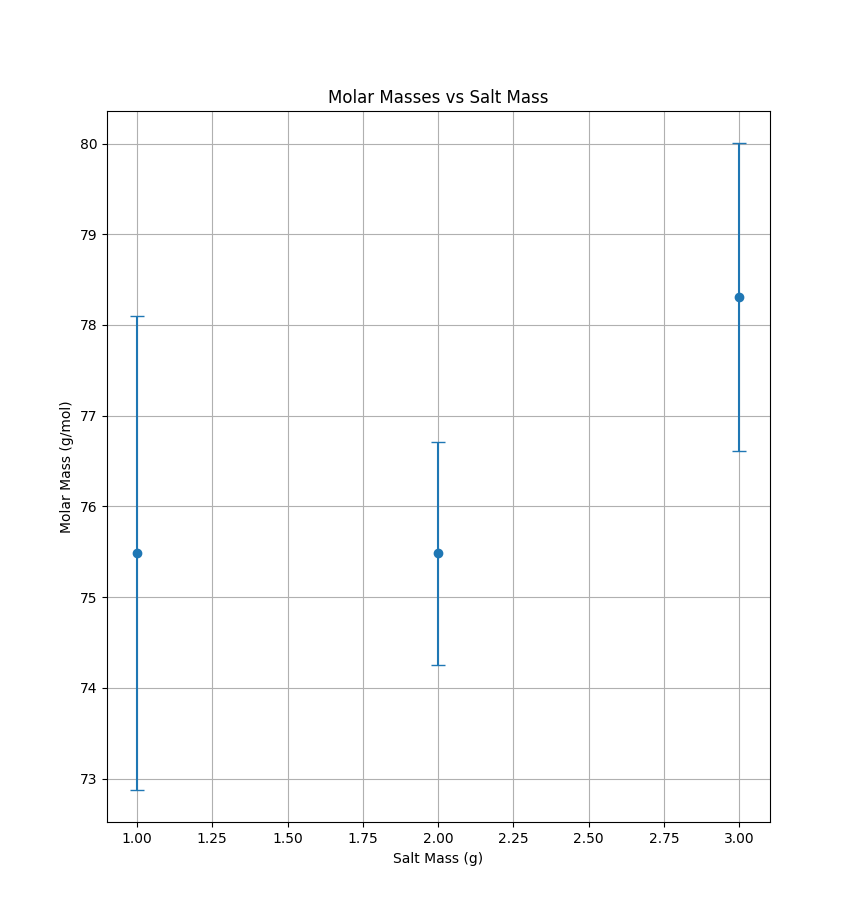
\includegraphics[width=\textwidth]{images/molar_mass_by_salt_mass.png}
    \caption{Molar mass of the salt as a function of the mass of salt used in the solution. Error bars indicate the uncertainties in the calculated molar masses.}
    \label{fig:molar_mass_plot}
\end{figure}

This plot demonstrates the consistency of the molar mass determination across different concentrations of the salt, with the molar mass remaining relatively constant despite variations in salt mass.

\section{Discussion}
The goal of this experiment was to determine the molar mass of a salt using the freezing point depression method. Our results yielded a mean molar mass of:
\begin{equation*}
M_{\text{mean}} = 76.5 \pm 1.0 \, \text{g/mol},
\end{equation*}
with a standard deviation of $1.64 \, \text{g/mol}$.

\subsection{Error Analysis}
The propagated error in our calculated mean molar mass was $1.0 \, \text{g/mol}$, while the standard deviation of the molar mass values was $1.64 \, \text{g/mol}$. The fact that the standard deviation is larger than the propagated error indicates some variability in the measurements beyond what was expected from error propagation alone.

Interestingly, this variability was entirely due to the measurement at the highest concentration (3~g of salt), as the calculated molar masses for the 1~ g and 2~g samples were identical within the significant digits. This suggests that the cryoscopic method's accuracy improves as the solute-to-solvent mass ratio approaches zero, which aligns with theoretical expectations that the method is most reliable at low concentrations.

While this behavior supports the notion that the observed deviation at higher concentrations is a consequence of the limitations inherent in the cryoscopic calculation formula, other factors might have also contributed to this variability, such as:
\begin{itemize}
    \item Slight variations in the actual temperature of the cooling bath during measurements,
    \item Minor inaccuracies in weighing the salt or solvent,
    \item Potential supercooling effects leading to slight differences in observed freezing points.
\end{itemize}

Overall, the relatively close agreement between the standard deviation and the propagated error suggests that our experimental setup and error analysis were reasonably reliable, even though the method's limitations at higher solute concentrations were evident in the 3 g measurement.


In addition to this, a more detailed examination of the relative errors reveals that the device error in measuring the freezing points is the dominant contributor to the overall uncertainty. Specifically, the relative errors on the measured freezing point differences, calculated using only the device error, were:
\[
\text{Relative Errors} = \begin{cases} 
0.020 & \text{for 1 g} \\
0.015 & \text{for 2 g} \\
0.010 & \text{for 3 g}
\end{cases}
\]
By comparison, the relative error on the final calculated molar mass was $0.012$. This clearly shows that the measurement error of the freezing point differences dominates the overall error in the experiment.

Therefore, the precision of the temperature measurement device used to measure the freezing points is the bottleneck in achieving more accurate results. For a more precise determination of the molar mass, improving the accuracy of this device would be crucial.

\subsection{Comparison with Potassium Chloride}
The molar mass obtained, $76.5 \, \text{g/mol}$, is close to that of potassium chloride (KCl), which has a molar mass of $74.55 \, \text{g/mol}$\footnote{Haynes, W. M. (Ed.). (2016). \textit{CRC Handbook of Chemistry and Physics} (97th ed.). CRC Press.}. However, the measured value lies outside the error margin of $\pm 1.0 \, \text{g/mol}$ for our overall experiment, indicating a statistically significant deviation from the literature value.

Interestingly, for the two lower salt concentrations (1 g and 2 g), the calculated molar mass was $75.6 \, \text{g/mol}$, which places the literature value almost within the error margin for these cases. This suggests that the observed discrepancy might be due to the inherent limitations of the cryoscopic method, particularly at higher solute-to-solvent mass ratios.

The cryoscopic calculation formula assumes an ideal solution, which becomes less accurate as the solute-to-solvent mass ratio increases. Given that this ratio approaches zero in our lower concentration measurements, the result aligns more closely with the literature value, further supporting the identification of the salt as KCl or a very similar compound.

Therefore, while the overall molar mass determination deviates slightly from the expected value, the results at lower concentrations support that the salt used in the experiment was likely potassium chloride. The experiment was thus successful in both determining the molar mass of the unknown salt and identifying it as KCl.

\subsection{Conclusion}
The experiment effectively demonstrated the freezing point depression method for determining the molar mass of an unknown salt. While there was some variability in the measurements, the final molar mass value was reasonably consistent with the known molar mass of potassium chloride, suggesting that the salt used was KCl or a similar compound. This outcome shows the utility of colligative properties in practical chemical analysis and reinforces the importance of careful measurement and error analysis in experimental chemistry.

\section{Acknowledgements and Disclosure}
This protocol was prepared with the assistance of ChatGPT, an AI language model developed by OpenAI. ChatGPT was used to generate sections of this document, including the introduction, methods, results, and discussion. All content generated by ChatGPT was thoroughly reviewed and, if necessary, modified by the authors before inclusion in the final protocol.

For transparency and reproducibility, all scripts used for data evaluation, the source code for this LaTeX document, and the conversations with ChatGPT are available online\footnote{The GitHub repository containing these resources can be accessed at: \url{https://github.com/kilianmandon/pc_praktikum/tree/main/freezing_point}. These resources will be accessible for up to four weeks after the conclusion of the lab course.}.

We acknowledge the role of AI in facilitating the preparation of this protocol while emphasizing the critical review and oversight by the authors to ensure accuracy and integrity in the presentation of this experiment.

\end{document}